% Regenerate: nix-shell -p texliveSmall poppler_utils --run "pdflatex gitops-workflow.tex && pdftocairo -svg gitops-workflow.pdf gitops-workflow.svg"
% lmodern matters: without it pdflatex emits bitmap fonts and the SVG text comes out rasterised.
\documentclass[border=10pt]{standalone}
\usepackage{tikz}
\usepackage{lmodern}
\usepackage[T1]{fontenc}
\usetikzlibrary{arrows.meta, positioning, fit, backgrounds, calc}

% Never black!N for anything outside a filled box: it vanishes on dark backgrounds.
\definecolor{ink}{HTML}{8A919C}

\begin{document}
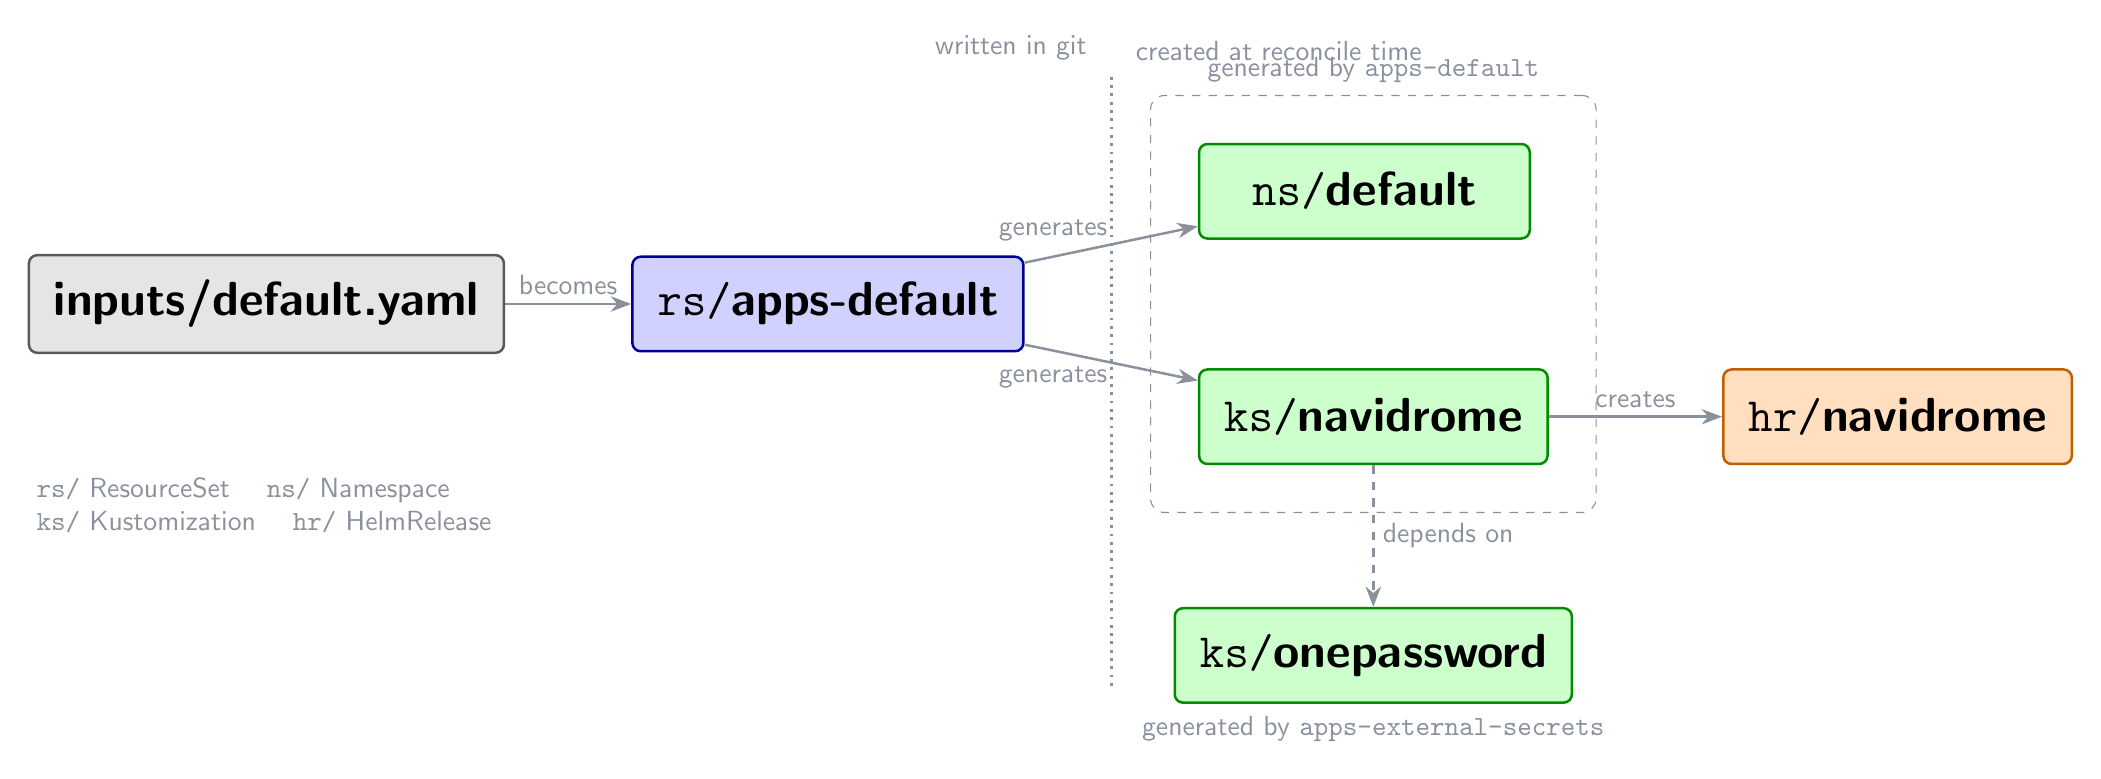
\begin{tikzpicture}[
  font=\sffamily\LARGE,
  node distance=14mm and 16mm,
  box/.style={
    rounded corners=3pt, draw, line width=0.9pt,
    align=center, inner sep=9pt, minimum width=42mm, minimum height=12mm
  },
  file/.style ={box, fill=gray!20,   draw=gray!70!black},
  rset/.style ={box, fill=blue!18,   draw=blue!60!black},
  ks/.style   ={box, fill=green!20,  draw=green!55!black},
  helm/.style ={box, fill=orange!25, draw=orange!75!black},
  flow/.style ={-{Stealth[length=2.6mm]}, draw=ink, line width=0.9pt},
  dep/.style  ={-{Stealth[length=2.6mm]}, draw=ink, line width=0.9pt, dashed},
  lbl/.style  ={font=\sffamily\normalsize, text=ink, inner sep=3pt}
]

\node[file] (a)                        {\textbf{inputs/default.yaml}};
\node[rset, right=of a] (b)            {\texttt{rs/}\textbf{apps-default}};

\node[ks, above right=2mm and 22mm of b] (n) {\texttt{ns/}\textbf{default}};
\node[ks, below right=2mm and 22mm of b] (c) {\texttt{ks/}\textbf{navidrome}};

\node[helm, right=22mm of c] (e)       {\texttt{hr/}\textbf{navidrome}};
\node[ks, below=18mm of c] (g)         {\texttt{ks/}\textbf{onepassword}};

\draw[flow] (a) -- node[lbl, above] {becomes} (b);
\draw[flow] (b) -- node[lbl, above left=-1mm] {generates} (n);
\draw[flow] (b) -- node[lbl, below left=-1mm] {generates} (c);
\draw[flow] (c) -- node[lbl, above] {creates} (e);
\draw[dep]  (c) -- node[lbl, right] {depends on} (g);

% The one thing a reader cannot guess: everything right of this line is
% created at reconcile time and is written down nowhere.
\begin{scope}[on background layer]
  \coordinate (mid) at ($(b.east)!0.5!(c.west)$);
  \draw[ink, dotted, line width=1pt] ($(mid)+(0,3.6)$) -- ($(mid)+(0,-4.2)$);
  \node[lbl, anchor=south east] at ($(mid)+(-2mm,3.7)$) {written in git};
  \node[lbl, anchor=south west] at ($(mid)+(2mm,3.7)$) {created at reconcile time};
\end{scope}

% The region is what mermaid cannot draw: it marks where one ResourceSet's
% output ends. onepassword sits outside it because another one generates it.
\begin{scope}[on background layer]
  \node[draw=ink, dashed, rounded corners=5pt,
        inner sep=6mm, fit=(n)(c)] (box) {};
  \node[lbl, anchor=south] at ($(box.north)+(0,0.5mm)$) {generated by \texttt{apps-default}};
  \node[lbl, below=0.5mm of g.south] {generated by \texttt{apps-external-secrets}};
\end{scope}

\node[lbl, anchor=north west, align=left] at ($(a.west)+(0,-2.1)$)
  {\texttt{rs/}~ResourceSet \quad \texttt{ns/}~Namespace\\
   \texttt{ks/}~Kustomization \quad \texttt{hr/}~HelmRelease};

\end{tikzpicture}
\end{document}
